\documentclass[a4paper]{llncs}
\usepackage[T1]{fontenc}
\usepackage[utf8]{inputenc}
\usepackage{lmodern}
\usepackage[scaled=.8]{beramono}
\usepackage{latexsym}
\usepackage{textcomp}

\usepackage{listings}
\lstset{numbers=left, captionpos=b, frame=single, basicstyle=\ttfamily, stringstyle=\small, breaklines=true, extendedchars=true, showstringspaces=true, numberbychapter=false}

\usepackage{graphicx}
\usepackage{multirow}
\usepackage{booktabs}
\usepackage{tabularx}
\usepackage{ctable}
\usepackage{array}
\usepackage{hyperref}
\usepackage{enumitem}
\setlist[itemize,enumerate]{leftmargin=*}

\def\sectionautorefname{Section}
%\renewcommand{\bibname}{References}

\begin{document}

\title{Decentralised Authoring, Annotations and Notifications for a Read-Write Web with dokieli}

\author{Sarven Capadisli\inst{1}
  \and Amy Guy\inst{2}
  \and Ruben Verborgh\inst{3}
  \and Christoph Lange\inst{1,4}
  \and Sören Auer\inst{1,4}
  \and Tim Berners-Lee\inst{5}}
\institute{%
  University of Bonn, Bonn, DE
  \email{info@csarven.ca, \{langec,auer\}@cs.uni-bonn.de}
  \and School of Informatics, University of Edinburgh, Edinburgh, UK
  \email{amy@rhiaro.co.uk}
  \and Ghent University – \empty imec, Ghent, BE
  \email{ruben.verborgh@ugent.be}
  \and Fraunhofer IAIS, Sankt Augustin, DE
  \and Decentralized Information Group, CSAIL, MIT, Cambridge, US
  \email{deiu@mit.edu, timbl@w3.org}
}
\maketitle

\begin{abstract}
  While the Web was designed as a decentralised environment, individual authors still lack the ability to conveniently author and publish documents, and to engage in social interactions with documents of others in a truly decentralised fashion. We present \textit{dokieli}, a fully decentralised, browser-based authoring and annotation platform with built-in support for social interactions, through which people retain the ownership of and sovereignty over their data. The resulting “living” documents are interoperable and independent of dokieli since they follow standards and best practices, such as HTML+RDFa for a fine-grained semantic structure, Linked Data Platform for personal data storage, and Linked Data Notifications for updates. This article describes dokieli’s architecture and implementation, demonstrating advanced document authoring and interaction without a single point of control. Such an environment provides the right technological conditions for independent publication of scientific articles, news, and other works that benefit from diverse voices and open interactions. To experience the described features please open this document in your Web browser under its canonical URI: {\tt \href{http://csarven.ca/dokieli-rww}{http://csarven.ca/dokieli-rww}}.
  \keywords{Decentralisation, Human-computer interaction, Linked Data, Semantic publishing, Social machine, Social web}
\end{abstract}


\section{Introduction}
\label{introduction}

\par While the Web was originally conceived as a decentralised platform where every organisation and individual can participate, it became increasingly centralised with \empty less than 1\% of the servers serving more than 99\% of the content. The main reason for this is rooted in technology: it is currently much easier and more efficient to author, manage, publish, and search large amounts of similarly structured content using a centralised platform. Blogger, YouTube and Facebook, for example, are centralised authoring, publishing, and search platforms for blog posts, videos or social network content respectively.

\par However, independence of centralised platforms is a necessity for ownership of published ideas, and to establish a relation of trust. For example, Facebook has been accused of bias, false information, and censorship—but rather than blaming this on any particular platform, we identify it as an unavoidable result of centralisation. After all, there is a continued tension between unrestricted publication rights on the one hand, and a guarantee of balanced, verified information on the other. In a fully decentralised setting, each source is filterless and responsible for its own quality and reputation, while others are free to selectively (dis-)trust certain sources using any mechanism they desire.

\par Decentralised authoring, publication, and annotation furthermore have the potential to impact areas in which centralisation currently determines the pace of evolution. Scientific publishing, for instance, is often bound to centralised review and dissemination processes. Instead, rigorous scientific discourse could be realised with an open, decentralised environment for the annotation of manuscripts, which has the potential to engage more people sooner. Trust then no longer stems from a finite process with limited transparency, but is rather continuously assessed by repeated independent validation. Publication thereby becomes the starting point rather than the end point.

\par If we want to strengthen the decentralised nature of the Web again, we need to develop technologies to simplify the decentralised authoring, management, exploration, and search of Web content.

\par In this article we present the principles and architecture for a fully distributed authoring and publishing system in Sections 2 and 4 respectively. We describe the dokieli implementation of this architecture as well as an overview on its current adoption in Section 5 before we conclude with an outlook on challenges and future work in Section 6.

\section{Principles}
\label{principles}

\par This describes the principles against which decentralised approaches for authoring, annotation and notifications should be designed. These principles are derived from current literature on decentralisation, and Web development best practices.

\par \textbf{Data storage independent of service providers}: Users should have a choice in where they store their data and full control over it e.g. with regard to who is allowed to access it. The \textit{Industrial Data Space}~\cite{ref-1} initiative calls this ``data sovereignty''.

\par \textbf{Interoperability}: By allowing the application logic to be decoupled from the data, users can switch between applications and personal data storage servers, thereby avoiding a \textit{vendor lock-in}. To achieve maximum interoperability, applications should conform to well-defined Web standards and protocols (rather than properietary software implementations). Dangers of data silos and some example standards to use to decentralise are given in \textit{Socially-aware Cloud Storage}~\cite{ref-2}.

\par \textbf{Separation of concerns}: A \textit{progressive enhancement} strategy to connect the structural, presentational, and behavioural layers allows content and base functionality to be accessible through different media and devices (as described in \textit{Progressive Enhancement and the Future of Web Design}~\cite{ref-3}).

\par \textbf{Accessibility}: To lower the barrier for entry for all forms of participation, enhanced functionality should be accessible to users based on the capabilities of their user-agents, storage availability, network access or personal preferences (we consider this to be self-evident, and there are a plethora of Web best practices in this area).

\par \textbf{Freedom of expression}: Because there are no central authorities, we must assume applications follow the open-world principle, where ``any author can say anything about anything''. Identifying everything using [de]referenceable IRIs allows any distributed authoring or annotation application to reference and link to previously published content (this overlaps with Principles 1, 3 and 4 in the \textit{W3C Semantic Web Activity}~\cite{ref-4} charter.

\par \textbf{Web of Trust}: The Web as a collaborative medium makes it possible for people to take responsibility (or be accountable) for their contributions. It should be possible for people to publish, share, and annotate information while ensuring their provenance, authenticity and integrity ~\cite{ref-5,ref-6,ref-7}.


\section{Related Work}
\label{related-work}
                          
\par \textit{User Interfaces for Semantic Authoring of Textual Content}~\cite{ref-8} gives an overview on relevant related work. A range of quality attributes such as collaboration, interoperability, and scalability, while relevant to our work, we also consider systems and tools on dimensions based on the principles that we have outlined.

                            
\par 
                                \textbf{Centralised authoring and annotation platforms}:
                                \textit{Google Docs}, \textit{Medium}, and \textit{Authorea} are examples of Web applications for collaborative creation and publication of content which require account creation and data storage with respective centralised services. They allow multiple participants to annotate and hold discussions around the primary content; users must access their accounts to be notified of updates to conversations, and data from both the main content and related discussion is confined to the service which was used to create it.

                                \textit{WordPress} is a free and open-source platform for article publication which can be self-hosted on a server controlled by the user. Visitors may sign-in with their WordPress accounts to leave comments on others’ articles, however they are typically under the hosting site’s database.

                                \textit{Hypothesis} makes it possible for users to leave annotations on different types of documents on the Web using a browser plugin or via a proxy. Annotations may be private or public, and can be threaded to form conversations around a piece of content. Despite allowing the attachment of annotations to resources hosted anywhere, they depend on centralised account creation and storage for the annotations themselves. Hypothesis is open source, with an API that uses Web Annotations data model, and may be self-hosted, but currently it is not possible to federate between different instances.

                                \textit{Pundit} is a set of tools that allow web annotation with highlights, comments and semantic annotations. It is similar to hypothes.is in its architecture and deployment, i.e., annotations made through the pundit client require it to be saved on its corresponding annotations server.




                            

                            
\par 
                                \textbf{Decentralised authoring and annotation systems}:
                                Some authoring and publishing systems already go into a decentralised direction. However, they only realize a relatively small subset of the principles outlined in the last section. \textit{LibreOffice Online}, for example, allows collaborative editing of office documents (e.g., Writer) from the Web browser. Content can be stored under different CMSs in the cloud. The document’s interface consists of image tiles which are sent from the server and rendered in the browser. However, it hardly provides accessibility, rich interlinking and annotations or separations of concerns.

                                The \textit{Smallest Federated Wiki} pages to be forked and maintain personal copies.

                                

                                \textit{Amaya} is a desktop Web editor application (to create and update documents) as well as a lightweight browser that was (1993) developed by W3C to provide a framework to test its technologies.
                            

                            
\par The tools which provide good collaborative editing UIs appear to do so at the expense of data ownership and interoperability; those which promote creation and publication of data in open reusable formats are lacking facilities for linking discourse and conversation to concepts published. Decentralised creations also mean that each author can choose their own semantics (e.g. their own vocabulary to annotate RDF), and then such decentralised documents can link to each other and their schemas can also be mapped to each other, whereas in centralised platforms this is (if they support semantics at all) often prescribed, either technically enforced, or encouraged by social convention.
                        
                    

                    
                        \section{Architecture and technologies}
  \label{architecture-and-technologies}

                        
                            
\par In this section we discuss an architecture to bridge the gaps in existing work for a decentralised authoring and semantic annotation client-side application, which decouples itself from data and specific server requirements.

                            
                                \subsection{Architectural overview}
  \label{architectural-overview}

                                
                                    
\par Decentralised read-write environments make it possible for different actors (e.g., authors, reviewers) to have their own personal online storages where they can: manage their data; have socially-aware access controls on the data (e.g., who gets to see and update what); send notifications based on their interactions; and permit different applications to operate on the data, including moving the data from one server to another seamlessly. Figure ~\ref{fig:centralised-decentralised-architectures} depicts the contrast between typical centralised and decentralised architectures.

\begin{figure}
  \centering
  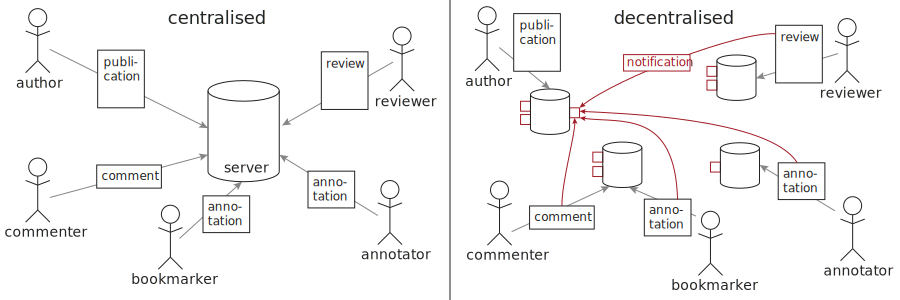
\includegraphics[width=\textwidth]{media/images/centralised-decentralised-architectures}
  \caption{Entities and relations within dokieli’s architecture}
  \label{fig:centralised-decentralised-architectures}
\end{figure}

\par dokieli as a client-side application can be \empty deployed on a single-page or through a browser extension, which can consume and interact with Linked Data anywhere on the Web. We consider an HTML document with embedded JavaScript as the default UI of a document. It is independent from specific server-side software, proprietary APIs or the requirement to have an account.

                                    
\par On the other hand, if desired and available, users can participate using their own profiles (WebIDs) located anywhere on the Web, and get to store and make their annotations in their own personal storage, as well as assign access controls to documents. Similarly, a decentralised communications protocol, \textit{Linked Data Notifications}~\cite{ref-9} (\textit{W3C Proposed Recommendation}~\cite{ref-10}), is used get past the limits of centralisation by enabling communication to happen across independent servers. Figure ~\ref{fig:dokieli-architecture-relations} depicts relations between the kinds of entities which underlay dokieli’s architecture, where nodes are under different domains and authority.

\begin{figure}
  \centering
  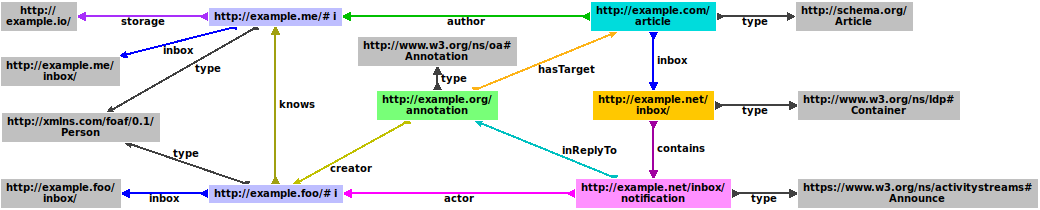
\includegraphics[width=\textwidth]{media/images/dokieli-architecture-relations}
  \caption{Typical centralised and decentralised architectures}
  \label{fig:dokieli-architecture-relations}
\end{figure}
                                    
\par dokieli is \textit{self-replicating}, in that the reader of a dokieli document can spawn an instance — either a copy or a brand new empty document — into their own storage space at the click of a button.

                            
                                \subsection{Creating documents}
  \label{creating-documents}

                                
                                    
\par Documents use HTML5 \textit{Polyglot Markup}~\cite{ref-11} to ensure that when served as (X)HTML respectively, they can be processed as either HTML or XML, which is useful in XML ecosystems and toolchains. Semantics is embedded directly into human-visible prose using RDFa. The machine-readable data is thus kept in context, reusing the article’s text as literal object values, and avoiding data duplication or data ‘islands’, which can occur when other RDF serialisations are included within HTML {\tt <script>} elements.
                                    

                                    
\par The appearance of documents is determined with CSS3. Different stylesheets can be applied to the same HTML structure so that a document can be presented flexibly, in the most appropriate way for a particular circumstance. Stylesheets can be switched from either dokieli’s menu or through Web browser with native controls, for example from a two-column layout required by an academic journal to a design in keeping with the author’s blog.

                                    
\par When JavaScript is enabled, dokieli provides a rich editing interface which includes visual and structural formatting of text as well as embedding machine-readable semantics, media, dynamic citations, and inclusion of statistical charts from live endpoints. An external personal data store, or even internet connection, are not needed at this stage as modifications to a document made in the browser this way can be persisted to a local filesystem using the dokieli menu \textit{export} function (or the browser’s \textit{save as}).
                                
                            

                            
                                \subsection{Consuming documents}
  \label{consuming-documents}

                                
                                    
\par Documents can be retrieved from Web servers with a single {\tt HTTP GET} request, by either a browser (for human-readable HTML) or script (machine-readable RDF). Through the use of progressive enhancement, document contents are available in text-only browsers, and further functionality of CSS and JavaScript are layered on according to the user agent’s abilities.

                                    
\par dokieli’s approach to marking human-visible content in RDFa makes it possible to further decouple itself, the application that produced the data, from the data itself, facilitating potential reuse of the data by other applications. A dokieli document can be parsed into a graph, and users can use any other RDF-aware application with the data that was generated by dokieli. Thereby, dokieli can effectively remove itself as a dependency when it comes to data consumption and reuse.

                                    
\par dokieli is able to authenticate users via WebID-TLS if they provide a WebID. This enables further functionality: the user can use dokieli to access protected resources and write to non-public data storage containers if their WebID is authorised to do so. For authenticated users leaving annotations on other documents dokieli fetches their name and display picture from their online profile if available, to display alongside their comment. 

                                    
\par dokieli uses the following vocabularies as standard: \textit{schema.org} to describe the general-purpose relations about the document as well as profiles, the \textit{SPAR Ontologies} for scholarly articles and referencing, \textit{Web Annotations} for annotations (with motivations e.g., replying, bookmarking, commenting, assessments), \textit{LDP} for personal storage management, \textit{WebAccessControl}/\textit{ACL} for access control, \textit{LDN Inbox} and \textit{ActivityStreams} for social notifications, \textit{Creative Commons} for rights and licensing, \textit{PROV Ontology} for provenance, and the \textit{RDF Data Cube vocabulary} to consume multi-dimensional data from SPARQL endpoints. Authors can optionally include other vocabularies to mark up specific concepts through dokieli’s UI.
                                
                            

                            
                                \subsection{Publishing documents}
  \label{publishing-documents}

                                
                                    
\par Documents can of course be published on ordinary Web servers, as ordinary Web pages. The next layer of enhancement is for authors who wish to edit documents on a Web server directly rather than locally; they can make use of dokieli’s write operations. This uses JavaScript, and moves the burden of processing user input from servers (i.e., offering HTML forms and processing of the form submission) to the client.  In essence, the expectation is that dokieli should be a ``smart client''.
                                    
                                    
\par dokieli implements the \textit{Linked Data Platform} (LDP) protocol for creating, updating and deleting documents. As such, personal data stores or servers which implement the server portion of the protocol can be used to store and edit dokieli documents directly. An {\tt HTTP PUT} request to a URL is used to create a \textit{new} document, to clone an existing one with \textit{save as}, to \textit{save} changes, and so that readers of a document can create their own document in \textit{reply}. All of these operations are available through the dokieli menu.
                                
                            

                            
                                \subsection{Social interactions and annotations}
  \label{social-interactions-and-annotations}

                                
                                    
\par Interactions with a document take the form of: a comment or (dis)like about the document as a whole, or an comment or (dis)like of a selection of text, i.e. an annotation. In both cases, the dokieli menu presents an input to the commenter, and then, adding additional semantic markup where necessary, sends the data off for appropriate storage so it can be retrieved and re-displayed on future document loads.

                                    
\par Document authors can point to a storage service (using the Web Annotations {\tt annotationService} property) which lets readers without their own personal storage comment nonetheless. Readers who have a preferred storage location against which they can authenticate are able to direct dokieli to store their input there instead (or in addition). Conforming to LDP, dokieli allows users to remove their annotations with an {\tt HTTP DELETE} operation. In this way, dokieli does not impose a centralised mechanism for social interactions, and allows users to effectively 'own' their comments, annotations, and reviews, in their own space..

                                    
                                
                            

                            
                                \subsection{Notifications}
  \label{notifications}

                                
                                    
\par When readers interact with a document, the author is notified by means of the \textit{Linked Data Notifications} (LDN) protocol. A notification, composed of the data from the interaction or annotation, is sent to the \textit{inbox} advertised by the document or arbitrary parts, thereof. This inbox may be on the same server as the document itself, or may be elsewhere. dokieli subsequently reads this inbox to display interactions and annotations on the document.

                                    
\par As the \textit{author} of the document has control of the inbox, they can remove notifications for interactions they find inappropriate, \textit{without} needing to worry about their inability to access the original source of the interaction. Conversely, annotators do not lose control or authority over their contributions, even if the object of their interaction wishes to disassociate itself. Each contributor retains their own respective rights over the entities they create on the Web.
                                
                            
                        
                    

                    
                        \section{Implementation}
  \label{implementation}

                        
                            
\par dokieli is open source: \url{https://github.com/linkeddata/dokieli} and available to try at \url{https://dokie.li/} (or at any instance on the Web, see \empty Adoption).

                            
                                \subsection{Components}
  \label{components}

                                
                                    
\par dokieli’s components include data (for structure and semantics), stylesheets (for presentation) and scripts (for interaction). All data (articles, annotations, notifications) are represented in HTML and RDF with vocabularies expressing the underlying content, resources are \textit{self-descriptive} to increase their reuse, and contain relations to related external resources to foster \textit{follow-your-nose} type of exploration.

                                    
\par Several stylesheets provide alternative views for consumption (e.g., stylesheets for different media: screens, print, slideshow). dokieli’s JavaScript includes: a library for editing (\textit{MediumEditor}) in its \textit{authoring environment}; features to \textit{fetch and display statistical data} from SPARQL endpoints (\textit{Sparqlines}~\cite{ref-12}); retrieval of profile information, as well as means to \textit{sign in} with \textit{WebID Authentication over TLS}~\cite{ref-13}; functionality for write-operations, which includes checking \textit{authorisation} against access-control level settings on the server with the authenticated user’s WebID and personal certificate; creation and consumption of \textit{Web Annotations} and \textit{Linked Data Notifications}; and fetching information from remote articles when adding a citation.

                                    
\par The scope of dokieli includes documents and the interactions around them. The creation and maintenance of user profiles, personal storage spaces, and access control rules are not managed by dokieli; since they are all standard mechanisms, users are expected to be able to accomplish this using other specialised applications.
                                
                            

                            
                                \subsection{Deployment}
  \label{deployment}

                                
                                    
\par dokieli employs two complementary deployment approaches: \textit{single-page application} and \textit{Web browser extension}.

                                    
\par dokieli’s presentational and behavioural code layers can be included in Web pages in order to trigger them as active single-page applications. It is a smart client that allows different kinds of articles e.g., academic, blog posts, news, to be authored and annotated from within Web browsers, without necessarily having them deployed from a server, i.e., it can be used offline or on localhost. dokieli internally handles its content and well-formed structural and semantic representation based on user’s interactivity. Articles, profiles and their contact information, notifications, annotations with different motivations, for instance, can be read and written ubiquitously to any Web space with standard LDP and access control mechanisms.

                                    
\par The Web browser extension is a thin wrapper around dokieli’s core code in order to embed itself in any HTML-based Web page on the Web. It inherits all of the features of a single-page application. While HTML based documents on the Web vary in their quality, dokieli’s write operations generate well-formed HTML+RDFa. One of the primary utilities for the extension is to have a consistent interface for annotating (comment, bookmark, like) any text selection on a Web page, as well as sharing parts of pages with ones contacts via notifications, without having a service dependency or being limited by the Web page’s UI.
                                
                            

                            
                                \subsection{Interactions}
  \label{interactions}

                                
                                    
\par Screencasts for the following use-cases showcase dokieli’s social features where users interact by creating and sharing information are at \url{https://dokie.li/}.

\begin{figure}
  \begin{minipage}[b]{.49\textwidth}
    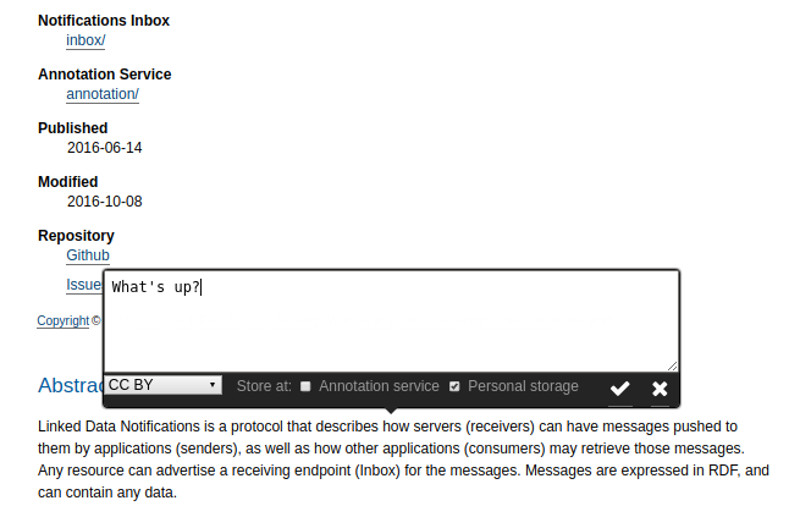
\includegraphics[width=\textwidth]{media/images/dokieli-annotation}
    \caption{dokieli Web Annotation}
    \label{fig:dokieli-annotation}
  \end{minipage}
  \hfill
  \begin{minipage}[b]{.49\textwidth}
    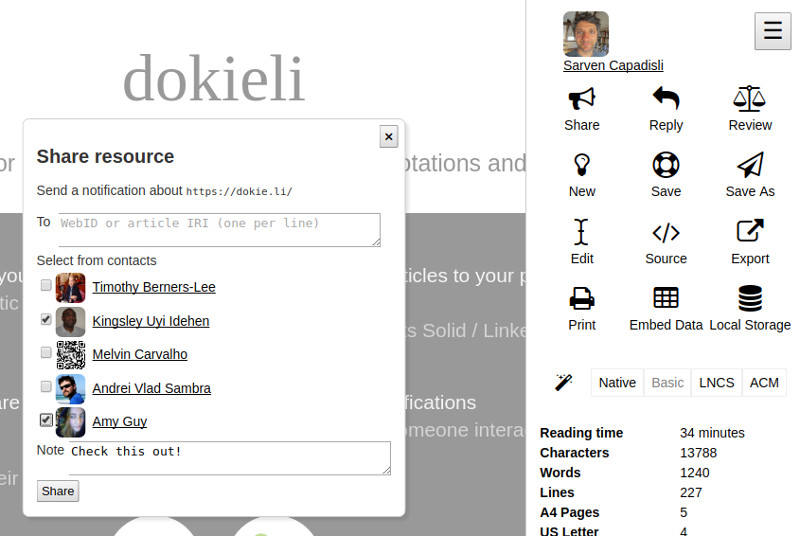
\includegraphics[width=\textwidth]{media/images/dokieli-share}
    \caption{dokieli Share}
    \label{fig:dokieli-share}
  \end{minipage}
\end{figure}
                                    

                                    
\par \textbf{Annotations}: A core feature to facilitate collaboration is the possibility to annotate arbitrary parts of a Web document.
                                    Users can select an entity or a span of text of interest, a context menu is presented to input their annotations along with the choice to select a license for their contribution.
                                    If the user is signed-in with their WebID, and provided they have a personal storage space, dokieli discovers this through their online profile and saves the annotations to that location.
                                    Once the annotation is submitted by the user, dokieli proceeds with three operations: 1) the annotation is requested to be saved at the user’s personal storage, and if it is access controlled, the user will be prompted to authenticate themselves against that server, before the annotation is saved and is assigned its own URL, 2) if the article or any identifiable statement or segment has its own inbox, dokieli sends a notification to the inbox indicating that an annotation was made and with its retrievable location, and accompanying metadata like who created it, date, its license etc., 3) the annotation is fetched from its canonical location, and integrated into the article e.g., in marginalia. If the article has a reference to a public annotation service (a writeable space adhering to \textit{Web Annotation Protocol}~\cite{ref-15}), the user has the option to send a copy of the annotation there as well. In cases where the user does not want to have the canonical copy of the annotation on their server, or if a user does not have write access to a storage, they can use this option to engage with the article.
                                    

                                    
\par \textbf{Social Sharing}: A key aspect of the Social Web is sharing with others.
                                    After (optionally) authenticating with a WebID, dokieli documents can be shared with contacts, which are discovered from the user’s WebID profile. Contacts whose profiles advertise an LDN Inbox will receive a notification of the share. The notification contains Activity Streams 2.0 vocabulary terms, and recipients can use any LDN-compatible application to view the notification, without needing to have ever used dokieli before.

\begin{figure}
  \begin{minipage}[b]{.53\textwidth}
    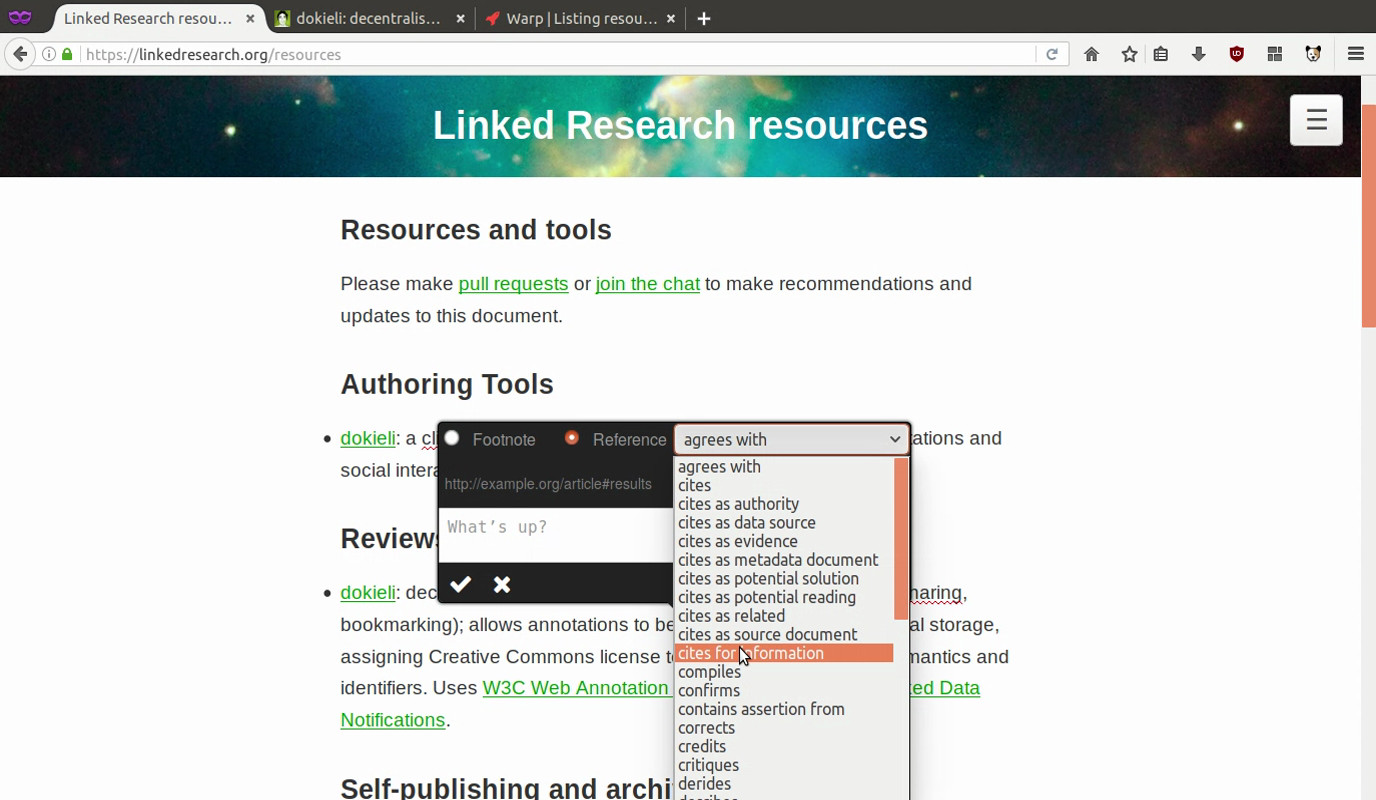
\includegraphics[width=\textwidth]{media/images/dokieli-citation}
    \caption{Semantic inline citations in dokieli}
    \label{fig:dokieli-citation}
  \end{minipage}
  \hfill
  \begin{minipage}[b]{.45\textwidth}
    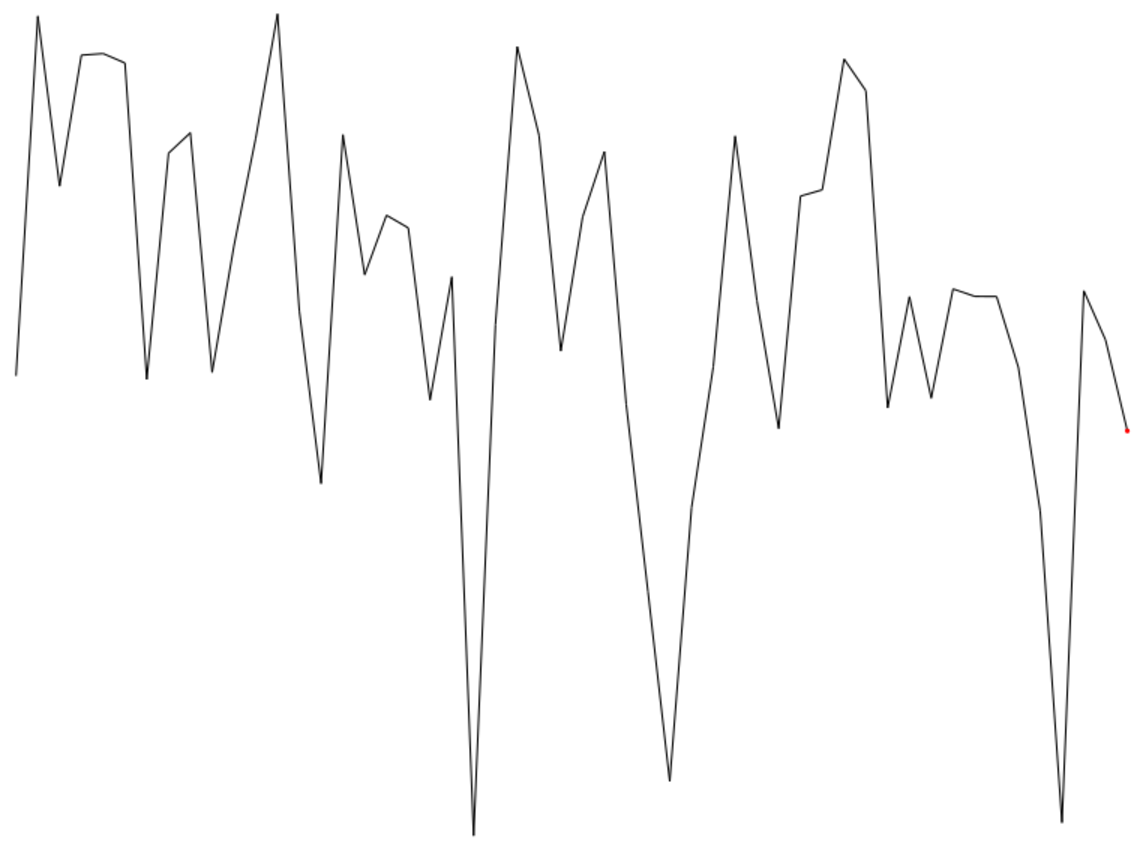
\includegraphics[width=\textwidth]{media/images/dokieli-sparqlines}
    \caption{Sparqlines interaction in dokieli}
    \label{fig:dokieli-sparqlines}
  \end{minipage}
\end{figure}


\par \textbf{Inline Citations}: Rich semantic links can also be established between dokieli documents themselves.
                                    The author selects a text fragment and inserts the URL of the document to be linked to as well as a semantic link type (e.g. “agrees with”, “confirms”, “cites as evidence”) from the CiTO and schema.org ontologies. dokieli automatically retrieves metadata (e.g. title, authors) from the linked document and adds a proper scientific endnote reference. If the linked document advertises a standard LDN Inbox, a notification of the citation is sent as well, thus allowing bi-directional linking.
                                    

                                    
\par \textbf{Statistical Data and Diagrams}: Embedding dynamically generated diagrams and charts is possible: after selecting text, the dokieli context menu offers results of a search across registered SPARQL endpoints for the keywords in the selected text, and presents a list of available data series to visualise. The result is an inline sparkline diagram.
                                
                            

                            
                                \subsection{Adoption}
  \label{adoption}

                                
                                    
\par The W3C Working Group Note \textit{Embedding Web Annotations}~\cite{ref-16} in HTML includes examples from dokieli’s use of the Web Annotation data \textit{Model}~\cite{ref-14} and \textit{Vocabulary}~\cite{ref-17} with motivations for example for ``Lightweight, decentralised Annotation Tools''.
                                    The \textit{Linked Data Notifications} specifications use dokieli’s HTML+RDFa template, and the \empty Editor’s Draft showcase dokieli as a consumer of LDN and Web Annotations. The LDN \empty tests suite also uses dokieli’s templates and stylesheets.

                                    
\par The academic workshop SemStats series use dokieli in its Website templates, including the call for contributions. CEUR-WS.org, an ``Online Proceedings for Scientific Conferences and Workshops'' offers the tooling ceur-make to help organisers generate proceedings using dokieli’s HTML+RDFa template.
                                    We list a community (of academics) who self-publish their articles and thesis using dokieli with different stylesheets and derived scripts under its examples in the wild. The conference series: WWW e.g., LDOW, WOW, ISWC, and ESWC propose dokieli as one tooling in which authors can use to for their contributions.

                                    
\par \url{https://linkedresearch.org/} uses dokieli in its templates on the site as well as workshop proposals and call for contributions.
                                    \url{http://csarven.ca/} uses dokieli in full, where some articles (like this article) offer pointers to a public annotation service in which users may wish to use for their annotations. Articles also dynamically embed annotations from personal storage spaces.
                                
                            
                        
                    

                    
                        \section{Conclusions}
  \label{conclusions}

                        
                            
\par 
                                The Web’s design stands out because of
                                its absence of centralised control,
                                both for technical reasons of scalability and resilience
                                as well as a societal need for freedom of expression.
                                A challenge in such large-scale decentralised networks
                                is how related publications can be semantically interlinked,
                                even if they are authored and published by different parties.
                                Centralising their publications is
                                practiced by the majority of authoring networks today,
                                demanding authors to give up some or all of their control
                                in exchange for technical simplicity.
                            
                            
\par 
                                dokieli shows
                                it is possible to build a social machine
                                wherein people interact with each other
                                without the need of centralised coordination.
                                Users can choose storage space for their content
                                independently of the applications with which they edit and view that content.
                                Documents are connected statically through links
                                and dynamically through Linked Data Notifications.
                                This is a proof for the viability of a decentralised authoring
                                and annotation environment built with Web standards.
                            
                            
\par 
                                On the other hand, dokieli’s use of standards
                                shows that dokieli itself is only one means to an end:
                                once the document has been created,
                                it lives on as an independent Web citizen.
                                The social machine consists of people and documents,
                                connected by Web standards,
                                with dokieli acting as just one possible catalyst.
                                Different Web applications can incorporate any of dokieli’s functions
                                and implement the principles to varying extents.
                                Since the data is loosely coupled to the application,
                                we avoid the \textit{walled garden} problem
                                of many current social platforms today.
                            
                            
\par 
                                A couple of important socio-technical challenges remain.
                                Resources might want to indicate in a granular way
                                which actions they support or encourage,
                                such as liking, bookmarking, or sharing,
                                and perhaps conditions about which notifications should be sent
                                when any of these events take place.
                                In order to encourage positive behaviour,
                                we might want ways to provide moderation,
                                and solutions to prevent harassment and abuse.
                                Closely related is the issue of identity, pseudonymity and anonymity,
                                and its relation with trust and verification.
                                While there is likely no final solution to these issues in an open ecosystem,
                                it is worthwhile exploring within dokieli or other tools.
                            
                            
\par 
                                Future work can examine how
                                additional features can be realised
                                on top of existing Web standards,
                                or where more development is required.
                                Real-time collaborative editing
                                is often realised with centralised communication
                                (even though some p2p alternatives exist).
                                Services like top-down annotations or automated entity marking
                                can improve the discoverability of a publication,
                                yet the question of how to offer these
                                without being tied to certain servers needs to be still solved. We invite you to try dokieli yourself. Annotate this article or spawn a new or a copy that you can edit yourself at \url{http://csarven.ca/dokieli-rww}.

                    
\paragraph{Acknowledgements:}
Special thanks to our colleagues at \empty MIT/\empty W3C; \empty Nicola Greco, \empty Dmitri Zagidulin, \empty Andrei Sambra, \empty Sandro Hawke, as well as \empty Henry Story and \empty Melvin Carvalho for their contributions. We are also thankful to collaborate with colleagues at \empty QCRI. This research was supported in part by \empty Qatar Computing Research Institute, \empty HBKU through the \empty Crosscloud project from 2015-10 to 2016-09. \empty Kingsley Idehen and \empty OpenLink Software for their support and contributions to the browser extension. Last but not least, the contributors to the dokieli code, issues, and discussion.

\begin{thebibliography}{99}
  \bibitem{ref-1} Otto, B., Auer, S., et al: Industrial Data Space, TR, 2016, \url{https://www.fraunhofer.de/content/dam/zv/en/fields-of-research/industrial-data-space/whitepaper-industrial-data-space-eng.pdf}
  \bibitem{ref-2} Berners-Lee, T.: Socially-aware Cloud Storage, 2009, \url{https://www.w3.org/DesignIssues/CloudStorage.html}
  \bibitem{ref-3} Champeon, S.: Progressive Enhancement and the Future of Web Design, 2003, \url{http://hesketh.com/publications/progressive\_enhancement\_and\_the\_future\_of\_web\_design.html}
  \bibitem{ref-4} Koivunen, M.-R., Eric Miller, E.: W3C Semantic Web Activity, 2001, \url{https://www.w3.org/2001/12/semweb-fin/w3csw}
  \bibitem{ref-5} Golbeck, J.: Weaving a Web of Trust, Science Magazine, Vol. 321, 2008, \url{https://pdfs.semanticscholar.org/5e37/daf945094ea9c9df127e06b05282e03e39bd.pdf}
  \bibitem{ref-6} Richardson, M., Agrawal, R., Domingos, P.: Trust Management for the Semantic Web, ISWC 2003, \url{https://link.springer.com/content/pdf/10.1007\%2F978-3-540-39718-2\_23.pdf}
  \bibitem{ref-7} Golbeck, J., Parsia, B., Hendler, J.: Trust Networks on the Semantic Web, LNCS 2782, Springer, 2003, \url{http://sir-lab.usc.edu/cs586/20151readings/w13-1.pdf}
  \bibitem{ref-8} Khalili, A., Auer, S.: User interfaces for semantic authoring of textual content: A systematic literature review, Web Semantics, Volume 22, pages 1–18 (2013), \url{http://svn.aksw.org/papers/2011/JWS\_SemanticContentAuthoring/public.pdf}
  \bibitem{ref-9} Capadisli, S., Guy, A., Lange, C., Auer, S., Deiu, A., Berners-Lee, T.: Linked Data Notifications: a resource-centric communication protocol, ESWC, 2017, \url{http://csarven.ca/linked-data-notifications}
  \bibitem{ref-10} Capadisli, S., Guy, A.: Linked Data Notifications, W3C Proposed Recommendation, 2017, \url{https://www.w3.org/TR/ldn/}
  \bibitem{ref-11} Graff, E., Silli, L.: Polyglot Markup: A robust profile of the HTML5 vocabulary, W3C Working Group Note, 2015, \url{https://www.w3.org/TR/html-polyglot/}
  \bibitem{ref-12} Capadisli, S.: Sparqlines: SPARQL to Sparkline, ISWC SemStats, 2016, \url{http://csarven.ca/sparqlines-sparql-to-sparkline}
  \bibitem{ref-13} Story, H., Corlosquet, S., Sambra, A.: WebID Authentication over TLS, W3C Editor’s Draft, 2014, \url{https://www.w3.org/2005/Incubator/webid/spec/tls/}
  \bibitem{ref-14} Sanderson, R., Ciccarese, P., Young, B.: Web Annotation Data Model, W3C Recommendation, 2017, \url{https://www.w3.org/TR/annotation-model/}
  \bibitem{ref-15} Sanderson, R.: Web Annotation Protocol, W3C Recommendation, 2017, \url{https://www.w3.org/TR/annotation-protocol/}
  \bibitem{ref-16} Cole, T., Capadisli, S., Young, B., Herman, I.: Embedding Web Annotations in HTML, W3C Working Group Note, 2017, \url{https://www.w3.org/TR/annotation-html/}
  \bibitem{ref-17} Sanderson, R., Ciccarese, P., Young, B.: Web Annotation Vocabulary, W3C Recommendation, 2017, \url{https://www.w3.org/TR/annotation-vocab/}
\end{thebibliography}

\end{document}
